Here we derive the Laplacian of a feed-forward NN with scalar output, that is $\Delta u \coloneqq \Tr(\gradsquared{\vx} u)$.
The goal is to make the dependence of the Laplacian w.r.t.\,a weight $\mW$ in one layer of the network explicit.
Then we can write down the Jacobian $\jac_{\mW}(\Delta u_{\vtheta})$ which is required for the Fisher used by energy NGD.

We first lay out the notation for feedforward neural networks, then use the ideas of Hessian backpropagation \citep[HBP,][]{dangel2020modular} to derive a recursion for the Hessian $\gradsquared{\vx}u_{\vtheta}$.
The Laplacian follows by taking the trace of the latter.
Finally, we express the Laplacians gradient w.r.t.
a single layer's weight $\mW$, i.e.\,$\nicefrac{\partial \Delta u_{\vtheta}}{\partial \mW}$, in terms of $\mW$'s children in the compute graph.

\subsubsection{Computing the input Hessian via backpropagation}

Gradient backpropagation describes a recursive procedure to compute gradients by backpropagating a signal via vector-Jacobian products (VJPs).
A similar procedure can be derived to compute Hessians w.r.t.\,nodes in a graph ($\vz^{(i)}$ or $\vtheta^{(i)}$).
We call this recursive procedure Hessian backpropagation~\citep{dangel2020modular}.

In the following, we set $C = 1$, that is the neural network produces a scalar $u$.

\paragraph{Gradient backpropagation} As a warm-up, let's recall how to compute the gradient $\grad{\vtheta}u =
(\grad{\vtheta^{(1)}} \dots \grad{\vtheta^{(L)}})$. We start by setting $\grad{u}
u = 1$, then backpropagate the error via VJPs,
\begin{align}\label{eq:gradient-backpropagation}
  \begin{split}
    \grad{\vz^{(i-1)}}u
    &=
      \left( \jac_{\vz^{(i-1)}} \vz^{(i)} \right)^{\top} \grad{\vz^{(i)}}u\,,
    \\
    \grad{\vtheta^{(i)}}u
    &=
      \left( \jac_{\vtheta^{(i)}} \vz^{(i)} \right)^{\top} \grad{\vz^{(i)}}u\,
  \end{split}
\end{align}
for $i = L, \dots, 1$, and initialization $\grad{\vz^{(L)}}u = \grad{u}u = 1$ of the recursion.
This yields the gradients of $u$ w.r.t.\,all intermediate representations and parameters.

\paragraph{Hessian backpropagation}
Recall the Hessian chain rule
\begin{equation*}
  % D^2(f\circ g)(x) = D^2f(g(x))(\nabla g(x), \nabla g(x)) +
  \nabla^2 (f\circ g) = (J g)^\top\cdot \nabla^2 f(g) \cdot Jg + \sum_{k} (\nabla f)_k \cdot \nabla^2 g_k,
\end{equation*}
where $g_i$ dentotes the individual components of $g$, see~\cite{skorski2019chain}.
The recursion for computing Hessians of $u$
w.r.t.\,intermediate representations and parameters starts by initializing the
recursion with $\gradsquared{\vz^{(L)}}u = \gradsquared{u} u = 0$, then
backpropagates according to
\begin{align}\label{eq:hessian-backpropagation}
  \begin{split}
    \gradsquared{\vz^{(i-1)}}u
    &=
      \left( \jac_{\vz^{(i-1)}} \vz^{(i)} \right)^{\top}
      \gradsquared{\vz^{(i)}}u
      \left( \jac_{\vz^{(i-1)}} \vz^{(i)} \right)
      +
      \sum_{k=1}^{h^{(i)}}
      \left(
      \gradsquared{\vz^{(i-1)}} [\vz^{(i)}]_k
      \right)
      [\grad{\vz^{(i)}} u]_k\,,
    \\
    \gradsquared{\vtheta^{(i)}}u
    &=
      \left( \jac_{\vtheta^{(i)}} \vz^{(i)} \right)^{\top}
      \gradsquared{\vz^{(i)}}u
      \left( \jac_{\vtheta^{(i)}} \vz^{(i)} \right)
      +
      \sum_{k=1}^{h^{(i)}}
      \left(
      \gradsquared{\vtheta^{(i)}} [\vz^{(i)}]_k
      \right)
      [\grad{\vz^{(i)}} u]_k
  \end{split}
\end{align}
for $i = L, \dots, 1$.
The first term takes the incoming Hessian (w.r.t.\,a layer's output) and sandwiches it between the layer's Jacobian.
It can be seen as backpropagating curvature from downstream layers.
The second term adds in curvature introduced by the current layer.
It is only non-zero if the layer is non-linear.
For linear layers, convolutional layers, and ReLU layers, it is zero.

\begin{figure}[t]
  \centering
  \resizebox{\linewidth}{!}{%
    % Define styles of nodes in computation graph sketch
\tikzset{%
  % shared basic style
  basicNode/.style={%
    rectangle,%
    minimum width=5ex,%
    minimum height=3.5ex,%
    inner sep=0.3ex,%
    rounded corners,%
    draw=black,%
    thick,%
    fill opacity=0.3,%
    text opacity=1.0,%
  },%
  % style for nodes representing neural network parameters
  paramNode/.style={%
    basicNode,%
    fill=maincolor,%
  },%
  % style for nodes representing data
  inputNode/.style={%
    basicNode,%
    fill=secondcolor,%
  },%
  % style for nodes indicating a repetition
  dotsNode/.style={%
    basicNode,%
    draw opacity=0,%
  },%
  % style for nodes representing intermediates from the forward pass
  forwardNode/.style={%
    basicNode,%
    fill=thirdcolor,%
  },%
  % style for nodes representing intermediates from the gradient backpropagation
  gradientNode/.style={%
    basicNode,%
    fill=fourthcolor,%
  },%
  % style for nodes representing intermediates from the Hessian % backpropagation
  hessianNode/.style={%
    basicNode,%
    fill=fifthcolor,%
  },%
}%
%%% Local Variables:
%%% mode: latex
%%% TeX-master: "../main"
%%% End:

\begin{tikzpicture}
  % arrange nodes in a matrix
  \matrix [%
  row sep=5ex,%
  column sep=5.5ex,%
  ampersand replacement=\&,% in order to put this inside of a scalebox
  ]{%
    % neural network parameters
    \node {Parameters};
    \&
    \&
    \&
    \node [paramNode] (param-1) {$\vtheta^{(1)}$};
    \&
    \node [dotsNode] (param-2) {$\dots$};
    \&
    \node [paramNode] (param-3) {$\vtheta^{(i-1)}$};
    \&
    \node [paramNode] (param-4) {$\vtheta^{(i)}$};
    \&
    \node [dotsNode] (param-5) {$\dots$};
    \&
    \node [paramNode] (param-6) {$\vtheta^{(L)}$};
    \\
    % forward pass
    \node {Forward};
    \&
    \&
    \node [inputNode] (forward-0) {$\vx$};
    \&
    \node [forwardNode] (forward-1) {$\vz^{(1)}$};
    \&
    \node [dotsNode] (forward-2) {$\dots$};
    \&
    \node [forwardNode] (forward-3) {$\vz^{(i-1)}$};
    \&
    \node [forwardNode] (forward-4) {$\vz^{(i)}$};
    \&
    \node [dotsNode] (forward-5) {$\dots$};
    \&
    \node [forwardNode] (forward-6) {$u$};
    \\
    % gradients
    \node {Backward};
    \&
    \&
    \node [gradientNode] (gradient-0) {$\grad{\vx}u$};
    \&
    \node [gradientNode] (gradient-1) {$\grad{\vz^{(1)}}u$};
    \&
    \node [dotsNode] (gradient-2) {$\dots$};
    \&
    \node [gradientNode] (gradient-3) {$\grad{\vz^{(i-1)}}u$};
    \&
    \node [gradientNode] (gradient-4) {$\grad{\vz^{(i)}}u$};
    \&
    \node [dotsNode] (gradient-5) {$\dots$};
    \&
    \node [gradientNode] (gradient-6) {$\grad{u}u$};
    \\
    % Hessians
    \node {Hess.\,backward};
    \&
    \node [hessianNode] (laplacian) {$\Delta u$};
    \&
    \node [hessianNode] (hessian-0) {$\gradsquared{\vx}u$};
    \&
    \node [hessianNode] (hessian-1) {$\gradsquared{\vz^{(1)}}u$};
    \&
    \node [dotsNode] (hessian-2) {$\dots$};
    \&
    \node [hessianNode] (hessian-3) {$\gradsquared{\vz^{(i-1)}}u$};
    \&
    \node [hessianNode] (hessian-4) {$\gradsquared{\vz^{(i)}}u$};
    \&
    \node [dotsNode] (hessian-5) {$\dots$};
    \&
    \node [hessianNode] (hessian-6) {$\gradsquared{u}u$};
    \\
  };
  % dependency arrows
  \foreach \i in {1,...,6} {
    \draw [-Latex, thick] (param-\i) to (forward-\i);
  }
  \foreach \i in {0,...,5} {
    \draw [-Latex, thick] (forward-\i) to (gradient-\i);
    \draw [-Latex, thick] (gradient-\i) to (hessian-\i);
    \draw [-Latex, thick, out=225, in=135] (forward-\i) to (hessian-\i);
  }
  \foreach \i in {0,...,5} {
    \pgfmathsetmacro{\j}{int(\i+1)}
    \draw [-Latex, thick] (forward-\i) to (forward-\j);
    \draw [-Latex, thick] (gradient-\j) to (gradient-\i);
    \draw [-Latex, thick] (hessian-\j) to (hessian-\i);
  }
  \foreach \i in {0,...,5} {
    \pgfmathsetmacro{\j}{int(\i+1)}
    \draw [-Latex, thick, out=215, in=45] (param-\j) to (gradient-\i);
    \draw [-Latex, thick, out=235, in=45] (param-\j) to (hessian-\i);
  }
  \draw [-Latex, thick] (hessian-0) to (laplacian);
\end{tikzpicture}
%%% Local Variables:
%%% mode: latex
%%% TeX-master: "../main"
%%% End:

  }
  \caption{Computation graph of a sequential neural network's Laplacian $\Delta u$ with $u \in \sR$.
    Arrows indicate dependencies between intermediates.
    Note that $\vz^{(0)} \coloneqq \vx$, $\vz^{(L)} \coloneqq u$, $\grad{u}u = 1$, and $\gradsquared{u}u = \vzero$.
    For the Gramian, we are interested in how the neural network parameters enter the Laplacian's computation.
    They are used during (i) the forward pass, (ii) the backward pass for the gradient, and (iii) the backward pass for the Hessian.}\label{fig:hbp-dependencies}
\end{figure}

Following the procedure of \Cref{eq:hessian-backpropagation} yields the
per-layer parameter and feature Hessians $\gradsquared{\vz^{(i)}}u,
\gradsquared{\vtheta^{(i)}}u$. In \Cref{fig:hbp-dependencies} we depict the dependencies of
intermediate gradients and Hessians for computing $\gradsquared{\vx}u_{\vtheta}$:
\begin{itemize}
\item $\grad{\vz^{(i-1)}}u$ depends on $\grad{\vz^{(i)}}u$ due to the recursion in \Cref{eq:gradient-backpropagation}, and on $\vz^{(i-1)}, \vtheta^{(i)}$ due to the Jacobian $\mJ_{\vz^{(i-1)}}\vz^{(i)}$ in the gradient backpropagation \Cref{eq:gradient-backpropagation}.

\item $\gradsquared{\vz^{(i-1)}}u$ depends on $\gradsquared{\vz^{(i)}}u$ and $\grad{\vz^{(i)}} u$ due to the recursion in \Cref{eq:hessian-backpropagation}, and on $\vz^{(i-1)}, \vtheta^{(i)}$ due to the Jacobian $\mJ_{\vz^{(i-1)}}\vz^{(i)}$ and Hessian $\gradsquared{\vz^{(i-1)}}[\vz^{(i)}]_k$ in the Hessian backpropagation \Cref{eq:gradient-backpropagation}.
\end{itemize}

% \subsection{Laplacian}

The Laplacian $\Delta u_{\vtheta}$ follows by taking the trace of
$\gradsquared{\vx}u_{\vtheta}$ from above, and is hence recursively defined.

\begin{figure}[t]
  \centering
  \begin{minipage}[b]{0.495\linewidth}
    \centering
    \resizebox{\linewidth}{!}{%
      % Define styles of nodes in computation graph sketch
\tikzset{%
  % shared basic style
  basicNode/.style={%
    rectangle,%
    minimum width=5ex,%
    minimum height=3.5ex,%
    inner sep=0.3ex,%
    rounded corners,%
    draw=black,%
    thick,%
    fill opacity=0.3,%
    text opacity=1.0,%
  },%
  % style for nodes representing neural network parameters
  paramNode/.style={%
    basicNode,%
    fill=maincolor,%
  },%
  % style for nodes representing data
  inputNode/.style={%
    basicNode,%
    fill=secondcolor,%
  },%
  % style for nodes indicating a repetition
  dotsNode/.style={%
    basicNode,%
    draw opacity=0,%
  },%
  % style for nodes representing intermediates from the forward pass
  forwardNode/.style={%
    basicNode,%
    fill=thirdcolor,%
  },%
  % style for nodes representing intermediates from the gradient backpropagation
  gradientNode/.style={%
    basicNode,%
    fill=fourthcolor,%
  },%
  % style for nodes representing intermediates from the Hessian % backpropagation
  hessianNode/.style={%
    basicNode,%
    fill=fifthcolor,%
  },%
}%
%%% Local Variables:
%%% mode: latex
%%% TeX-master: "../main"
%%% End:

\begin{tikzpicture}
  % arrange nodes in a matrix
  \matrix [%
  row sep=5ex,%
  column sep=5.5ex,%
  ampersand replacement=\&,% in order to put this inside of a scalebox
  ]{%
    % neural network parameters
    \&
    \&
    \node [dotsNode] (param-1) {$\dots$};
    \&
    \node [paramNode] (weight) {$\mW^{(i)}$};
    % \node [paramNode, anchor=west, xshift=0.5ex] (bias) at (weight.east) {$\vb^{(i)}$};
    \&
    \node [dotsNode] (param-3) {$\dots$};
    \\
    % forward pass
    \&
    \node [dotsNode] (forward-1) {$\dots$};
    \&
    \node [forwardNode] (forward-2) {$\vz^{(i-1)}$};
    \&
    \node [forwardNode] (forward-3) {$\vz^{(i)}$};
    \&
    \node [dotsNode] (forward-4) {$\dots$};
    \\
    % gradients
    \&
    \node [dotsNode] (gradient-1) {$\dots$};
    \&
    \node [gradientNode] (gradient-2) {$\grad{\vz^{(i-1)}}u$};
    \&
    \node [gradientNode] (gradient-3) {$\grad{\vz^{(i)}}u$};
    \&
    \node [dotsNode] (gradient-4) {$\dots$};
    \\
    % Hessians
    \node [hessianNode] (laplacian) {$\Delta u$};
    \&
    \node [dotsNode] (hessian-1) {$\dots$};
    \&
    \node [hessianNode] (hessian-2) {$\gradsquared{\vz^{(i-1)}}u$};
    \&
    \node [hessianNode] (hessian-3) {$\gradsquared{\vz^{(i)}}u$};
    \&
    \node [dotsNode] (hessian-4) {$\dots$};
    \\
  };
  % dependency arrows
  \foreach \i in {1,3} {
    \pgfmathsetmacro{\j}{int(\i+1)}
    \draw [-Latex, thick] (param-\i) to (forward-\j);
  }
  \foreach \i in {1,...,4} {
    \draw [-Latex, thick] (forward-\i) to (gradient-\i);
    \draw [-Latex, thick] (gradient-\i) to (hessian-\i);
    \draw [-Latex, thick, out=225, in=135] (forward-\i) to (hessian-\i);
  }
  \foreach \i in {1,...,3} {
    \pgfmathsetmacro{\j}{int(\i+1)}
    \draw [-Latex, thick] (forward-\i) to (forward-\j);
    \draw [-Latex, thick] (gradient-\j) to (gradient-\i);
    \draw [-Latex, thick] (hessian-\j) to (hessian-\i);
  }
  \foreach \i in {1,3} {
    \pgfmathsetmacro{\j}{int(\i)}
    \draw [-Latex, thick, out=215, in=45] (param-\i) to (gradient-\j);
    \draw [-Latex, thick, out=235, in=45] (param-\j) to (hessian-\j);
  }
  \draw [-Latex, thick] (hessian-1) to (laplacian);
  \draw [-Latex, ultra thick, secondcolor] (weight) to (forward-3);
  \draw [-Latex, ultra thick, secondcolor, out=215, in=45] (weight) to (gradient-2);
  \draw [-Latex, ultra thick, secondcolor, out=235, in=45] (weight) to (hessian-2);
\end{tikzpicture}
%%% Local Variables:
%%% mode: latex
%%% TeX-master: "../main"
%%% End:

    }
  \end{minipage}
  \hfill
  \begin{minipage}[b]{0.495\linewidth}
    \caption{Direct dependencies of a linear layer's weight matrix in the Laplacian's computation graph.
      There are three direct children: (i) The layer's output from the forward pass, (ii) the Laplacian's gradient w.r.t.\,the layer's input from the gradient backpropagation, and (iii) the Laplacian's Hessian w.r.t.\,the layer's input from the Hessian backpropagation.
      The gradients $\grad{\mW^{(i)}}\Delta u$ required for the Gramian are the vector-Jacobian products accumulated over those children.
    }\label{fig:laplacian-graph-weight}
  \end{minipage}
\end{figure}

\paragraph{Hessian backpropagation through nonlinear layers}
We mostly consider nonlinear layers without trainable parameters and consist of a componentwise nonlinearity $z\mapsto \sigma(z)$ for some $\sigma\colon\mathbb R\to\mathbb R$ and we assume $\sigma$ to be twice continuously differentiable (I guess one ask for weaker things).
The Jacobian of such a nonlinear layer is given by
\begin{equation}
  \jac_{\vz^{(i-1)}}\vz^{(i)} = \operatorname{diag}(\sigma'(\vz^{(i-1)}))
\end{equation}
and the %Hessian acts as
% \begin{equation*}
%   (\nabla^2_{\vz^{(i-1)}\vz^{(i)})(u,v) = u\odot v\odot \sigma''(z). %u^\top \operatorname{diag}(\sigma''(\vz_{i-1}))v = (v\top)
% \end{equation*}
Hessian terms are given by
\begin{equation}
  \nabla^2_{\vz^{(i-1)}}[\vz^{(i)}]_k = \sigma''(\vz^{(i-1)}_k) e_k  e_k^\top.
\end{equation}
\toodoo{Someone should definitely double check. I could not find a mistake -- MZ}
With these two identities we can backpropogate the input Hessian through the non-trainable nonlinear layers and obtain
\begin{equation}
  \gradsquared{\vz^{(i-1)}}u
  =
  \left( \operatorname{diag}(\sigma'(\vz^{(i-1)})) \right)^{\top}
  \gradsquared{\vz^{(i)}}u
  \left( \operatorname{diag}(\sigma'(\vz^{(i-1)})) \right)
  +
  \sum_{k=1}^{h^{(i)}}
  \operatorname{diag}(\sigma''(\vz^{(i-1)_k})
  e_k e_k^\top
  [\grad{\vz^{(i)}} u]_k\,,
\end{equation}

\paragraph{Hessian backpropagation through a linear layer} To de-clutter the dependency graph of \Cref{fig:hbp-dependencies}, we will now consider the dependency of $\Delta u_{\vtheta}$ w.r.t.\,the weight of a single layer.
We assume this layer $i$ to be a linear layer with parameters $\mW^{(i)}$ such that $\vtheta^{(i)} = \flatten(\mW^{(i)})$,
\begin{align}
  \vz^{(i)} = \mW^{(i)} \vz^{(i-1)}\,.
\end{align}
For this layer, the second terms in \Cref{eq:hessian-backpropagation} disappears because the local Hessians are zero, that is $\gradsquared{\vz^{(i-1)}}[\vz^{(i)}]_k = \vzero$ and $\gradsquared{\mW^{(i)}}[\vz^{(i)}]_k = \vzero$.
Also, the Jacobians are $\jac_{\mW^{(i)}}\vz^{(i)} = {\vz^{(i-1)}}^{\top} \otimes \mI$ and $\jac_{\vz^{(i-1)}}\vz^{(i)} = \mW^{(i)}$ and hence only depends on one of the two layer inputs.
This simplifies the computation graph.
\Cref{fig:laplacian-graph-weight} shows the dependencies of $\mW^{(i)}$ on the
Laplacian, highlighting its three direct children,
\begin{align}\label{eq:spatialDerivatives}
  \begin{split}
    \vz^{(i)}
    &=
      \mW^{(i)} \vz^{(i-1)}
    \\
    \grad{\vz^{(i-1)}}u
    &=
      {\mW^{(i)}}^{\top}
      \left(
      \grad{\vz^{(i)}}u
      \right)
    \\
    \gradsquared{\vz^{(i-1)}}u
    &=
      {\mW^{(i)}}^{\top}
      \left(
      \gradsquared{\vz^{(i)}}u
      \right)
      \mW^{(i)}
  \end{split}
\end{align}

\subsection{Computing the parameter derivative of the input Laplacian}
Recall, that the entries of the Fisher are composed from parameter derivatives of the input Laplacian, see~\eqref{eq:FisherInterior}.
Here, we only consider architectures where only the linear layers possess trainable parameters and therefore we compute the parameter $\partial_{\theta} \Delta u_\theta$ of the input Laplacian.

We have now identified the direct children of $\mW^{(i)}$ in the Laplacian's compute graph.
This allows us to write down its derivative $\grad{\mW^{(i)}} \Delta u$, which---by the chain rule---is simply the accumulated backpropagated error from the direct children:
\begin{align}\label{eq:laplacian-gradient}
  \begin{split}
    \grad{\mW^{(i)}} \Delta u_{\vtheta}
    &=
      \sum_{\bullet \in \left\{ \vz^{(i)}, \grad{\vz^{(i-1)}}u, \gradsquared{\vz^{(i-1)}}u \right\}}
      \left(
      \jac_{\mW^{(i)}}\bullet
      \right)^{\top}
      \grad{\bullet}\Delta u
    \\
    &=
      \left(
      \jac_{\mW^{(i)}}\vz^{(i)}
      \right)^{\top}
      \grad{\vz^{(i)}}\Delta u
      +
      \left(
      \jac_{\mW^{(i)}}\grad{\vz^{(i-1)}}u
      \right)^{\top}
      \grad{\grad{\vz^{(i-1)}}u}\Delta u
      +
      \left(
      \jac_{\mW^{(i)}}\gradsquared{\vz^{(i-1)}}u
      \right)^{\top}
      \grad{\gradsquared{\vz^{(i-1)}}u}\Delta u\,.
  \end{split}
\end{align}

% \paragraph{The Fisher}
With the Laplacian's gradient \Cref{eq:laplacian-gradient}, we can write down the Fisher block (up to summation over the data) for $\mW^{(i)}$ as
\begin{align}\label{eq:fisher}
  \begin{split}
    \mF^{(i)}
    &=
      \left(
      \grad{\mW^{(i)}} \Delta u_{\vtheta}
      \right)
      \left(
      \grad{\mW^{(i)}} \Delta u_{\vtheta}
      \right)^{\top}
    \\
    &=
      \sum_{\textcolor{blue}{\bullet} \in \left\{ \vz^{(i)}, \grad{\vz^{(i-1)}}u, \gradsquared{\vz^{(i-1)}}u \right\}}
      \sum_{\textcolor{red}{\bullet} \in \left\{ \vz^{(i)}, \grad{\vz^{(i-1)}}u, \gradsquared{\vz^{(i-1)}}u \right\}}
      \left(
      \left(
      \jac_{\mW^{(i)}}\textcolor{blue}{\bullet}
      \right)^{\top}
      \grad{\textcolor{blue}{\bullet}}\Delta u
      \right)
      \left(
      \left(
      \jac_{\mW^{(i)}}\textcolor{red}{\bullet}
      \right)^{\top}
      \grad{\textcolor{red}{\bullet}}\Delta u
      \right)^{\top}
    \\
    &=
      \sum_{\textcolor{blue}{\bullet} \in \left\{ \vz^{(i)}, \grad{\vz^{(i-1)}}u, \gradsquared{\vz^{(i-1)}}u \right\}}
      \sum_{\textcolor{red}{\bullet} \in \left\{ \vz^{(i)}, \grad{\vz^{(i-1)}}u, \gradsquared{\vz^{(i-1)}}u \right\}}
      \underbrace{
      \left(
      \jac_{\mW^{(i)}}\textcolor{blue}{\bullet}
      \right)^{\top}
      \left[
      \left(
      \grad{\textcolor{blue}{\bullet}}\Delta u
      \right)
      \left(
      \grad{\textcolor{red}{\bullet}}\Delta u
      \right)^{\top}
      \right]
      \left(
      \jac_{\mW^{(i)}}\textcolor{red}{\bullet}
      \right)}_{
      \coloneqq \mF^{(i)}_{\textcolor{blue}{\bullet}, \textcolor{red}{\bullet}}
      }\,.
  \end{split}
\end{align}

The Fisher consists of nine different terms.
Eventually, we would like to approximate it with a single Kronecker product, like KFAC~\citep{martens2015optimizing}.
\toodoo{We could either work with the diagonal terms, or if all terms admit Kronecker representations we could also approximate this sum of Kroneckers by the Kronecker of the sums...?}
We begin by studying the diagonal terms $\mF_{\textcolor{blue}{\bullet}, \textcolor{blue}{\bullet}}^{(i)}$ and call them zeroth, first and second order diagonal terms for $\textcolor{blue}{\bullet} = \vz, \nabla u, \nabla^2 u$, respectively.
\toodoo{Other question: might it be possible to write the nine terms as a Kronecker product of a sum of 3 matrices with a sum of 3 matrices?}

\paragraph{Computing $\mJ_{\mW^{(i)}}\textcolor{blue}{\bullet}$}
Let us first compute the Jacobians $\mJ_{\mW^{(i)}}\textcolor{blue}{\bullet}$ for which we envoke~\eqref{eq:spatialDerivatives}.
We already know the Jacobian from the linear layer's forward pass,
\begin{subequations}\label{eq:fisher-jacobians}
  \begin{align}
    \jac_{\mW}\left( \mW \vx \right) = \vx^{\top} \otimes \mI\,.
  \end{align}
  The Jacobian from the gradient backpropagation is
  \begin{align}
    \jac_{\mW}\left( \mW^{\top} \vx \right) = \mI \otimes \vx^{\top}\,,
  \end{align}
  and the Jacobian from the Hessian backpropagation is
  \begin{align}\label{subeq:fisher-jacobians-hbp}
    \jac_{\mW}\left( \mW^{\top} \mX \mW \right)
    =
    \mI \otimes \mW^{\top}\mX
    +
    \mK \left(
    \mI
    \otimes
    \mW^{\top}\mX^{\top}
    \right)\,,
  \end{align}
\end{subequations}
where $\mK \in \sR^{\dim(\mZ) \times \dim(\mZ)}$ (denoting $\mZ := \mW^{\top}\mX \mW$) is a permutation matrix that, when multiplied onto a vector whose basis corresponds to that of the flattened output $\mZ$, modifies the order from first-varies-fastest into last-varies-fastest, i.e.
\begin{equation*}
  \mK \flatten(\mZ) = \flatten(\mZ^{\top})\,.
\end{equation*}
Re-introducing the layer indices (\eqref{eq:spatialDerivatives}), this yields
\begin{align}
  \begin{split}
    \jac_{\mW^{(i)}}\vz^{(i)}
    &=
      {\vz^{(i-1)}}^\top\otimes \mI
    \\
    \jac_{\mW^{(i)}}\grad{\vz^{(i-1)}}u
    &=
      \mI\otimes
      \grad{\vz^{(i)}}u
    \\
    \jac_{\mW^{(i)}}\gradsquared{\vz^{(i-1)}}u
    &=
      \mI \otimes
      \left[
      {\mW^{(i)}}^{\top}
      \left(
      \gradsquared{\vz^{(i)}}u
      \right)
      \right]
      +
      \mK
      \left(
      \mI \otimes
      \left[
      {\mW^{(i)}}^{\top}
      \left(
      \gradsquared{\vz^{(i)}}u
      \right)^{\top}
      \right]
      \right)
  \end{split}
\end{align}
We will now use symmetries in the objects used during Hessian backpropagation to simplify those equations further.
At a first glance, it looks like the Fisher consists of 16 terms, as there are 4 terms from the Jacobians in \Cref{eq:fisher-jacobians}.
However, we can simplify into 9 terms:

First, $\gradsquared{\vz^{(i)}}u$ is symmetric, that is
\begin{align*}
  \jac_{\mW^{(i)}}\left( {\mW^{(i)}}^{\top} \left( \gradsquared{\vz^{(i)}}u  \right)\mW^{(i)} \right)
  &=
    \mI \otimes
    \left[
    {\mW^{(i)}}^{\top} \left( \gradsquared{\vz^{(i)}}u  \right)
    \right]
    +
    \mK
    \left(
    \mI \otimes
    \left[
    {\mW^{(i)}}^{\top}
    \left(
    \gradsquared{\vz^{(i)}}u
    \right)
    \right]
    \right)
    \shortintertext{and the transposed Jacobian is}
  &\mI \otimes
    \left[
    \left( \gradsquared{\vz^{(i)}}u  \right) \mW^{(i)}
    \right]
    +
    \left(
    \mI \otimes
    \left[
    \left(
    \gradsquared{\vz^{(i)}}u
    \right)
    \mW^{(i)}
    \right]
    \right)
    \mK^{\top}\,.
\end{align*}
Second, we multiply the transpose Jacobian onto $\grad{\gradsquared{\vz^{(i-1)}}u}\Delta u$, which inherits symmetry from the Hessian, $[\grad{\gradsquared{\vz^{(i-1)}}u}\Delta u]_{j,k} = [\grad{\gradsquared{\vz^{(i-1)}}u}\Delta u]_{k,j}$.
Due to this symmetry, the action of $\mK$ (or $\mK^{\top}$) does not alter it,
\begin{align*}
  \mK^{\top}\left( \grad{\gradsquared{\vz^{(i-1)}}u}\Delta u \right) = \grad{\gradsquared{\vz^{(i-1)}}u}\Delta u\,.
\end{align*}
In other words, it does not matter how we flatten (first- or last-varies-fastest).
This simplifies the VJP to
\begin{align*}
  \left(
  \mI \otimes
  \left[
  \left( \gradsquared{\vz^{(i)}}u  \right) \mW^{(i)}
  \right]
  \right)
  \grad{\gradsquared{\vz^{(i-1)}}u}\Delta u
  +
  \left(
  \mI \otimes
  \left[
  \left(
  \gradsquared{\vz^{(i)}}u
  \right)
  \mW^{(i)}
  \right]
  \right)
  \mK^{\top}
  \grad{\gradsquared{\vz^{(i-1)}}u}\Delta u
  =
  2 \left(
  \mI \otimes
  \left[
  \left( \gradsquared{\vz^{(i)}}u  \right) \mW^{(i)}
  \right]
  \right)
  \grad{\gradsquared{\vz^{(i-1)}}u}\Delta u
  \,.
\end{align*}
We can now write down the gradient from \Cref{eq:laplacian-gradient}, whose
self-outer product forms the Gramian for a linear layer, as
\begin{align*}
  \begin{split}
    \grad{\mW^{(i)}} \Delta u_{\vtheta}
    &=
      \underbrace{
      \left(
      {\vz^{(i-1)}}^\top\otimes \mI
      \right)^{\top}
      \grad{\vz^{(i)}}\Delta u
      }_{(1)}
      +
      \underbrace{
      \left(
      \mI \otimes \grad{\vz^{(i)}}u
      \right)^{\top}
      \grad{\grad{\vz^{(i-1)}}u}\Delta u
      }_{(2)}
      +
      \underbrace{
      2
      \left(
      \mI \otimes
      \left[
      \left( \gradsquared{\vz^{(i)}}u \right) \mW^{(i)}
      \right]
      \right)
      \grad{\gradsquared{\vz^{(i-1)}}u}\Delta u
      }_{(3)}
      \,,
  \end{split}
\end{align*}
where (1) is the contribution from the forward pass, (2) is the contribution from the gradient backpropagation, and (3) is the contribution from the Hessian backpropagation.

\begin{figure}[t]
  \centering
  Full interior Gramian\\
  \includegraphics[width=0.43\linewidth]{kfac_pinns_exp/exp04_gramian_contributions/fig/gram_full.png}

  \begin{tabular}{ccc}
    (\textcolor{blue}{forward}, \textcolor{red}{forward})
    &
      (\textcolor{blue}{forward}, \textcolor{red}{gradient})
    &
      (\textcolor{blue}{forward}, \textcolor{red}{Hessian})
    \\
    
\includegraphics[width=0.22\linewidth]{kfac_pinns_exp/exp04_gramian_contributions/fig/gram_output_output.png}
    &
      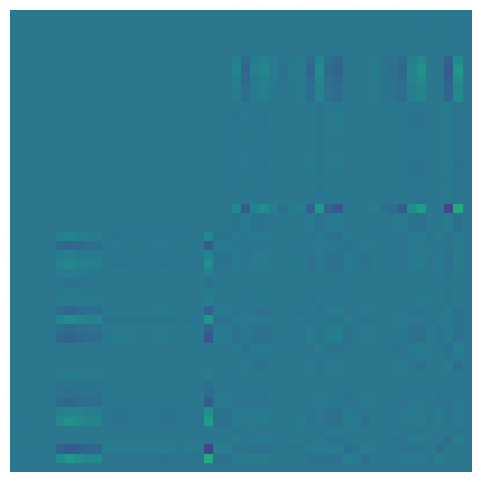
\includegraphics[width=0.22\linewidth]{kfac_pinns_exp/exp04_gramian_contributions/fig/gram_output_grad_input.png}
    &
      
\includegraphics[width=0.22\linewidth]{kfac_pinns_exp/exp04_gramian_contributions/fig/gram_output_hess_input.png}
    \\
    (\textcolor{blue}{gradient}, \textcolor{red}{forward})
    &
      (\textcolor{blue}{gradient}, \textcolor{red}{gradient})
    &
      (\textcolor{blue}{gradient}, \textcolor{red}{Hessian})
    \\
    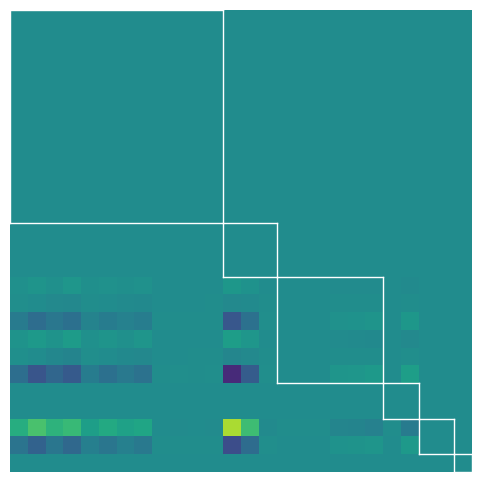
\includegraphics[width=0.22\linewidth]{kfac_pinns_exp/exp04_gramian_contributions/fig/gram_grad_input_output.png}
    &
      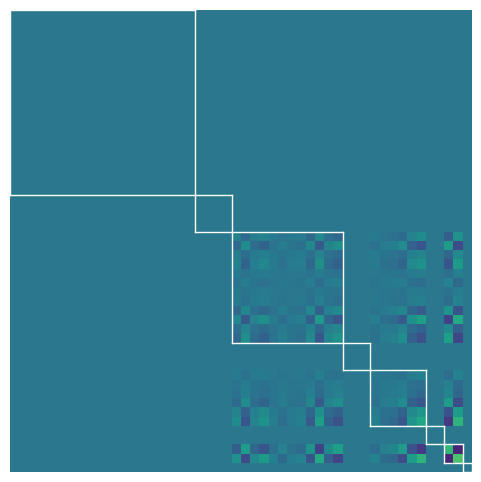
\includegraphics[width=0.22\linewidth]{kfac_pinns_exp/exp04_gramian_contributions/fig/gram_grad_input_grad_input.png}
    &
      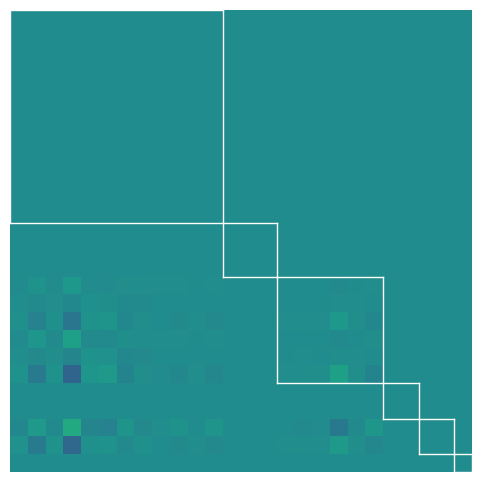
\includegraphics[width=0.22\linewidth]{kfac_pinns_exp/exp04_gramian_contributions/fig/gram_grad_input_hess_input.png}
    \\
    (\textcolor{blue}{Hessian}, \textcolor{red}{forward})
    &
      (\textcolor{blue}{Hessian}, \textcolor{red}{gradient})
    &
      (\textcolor{blue}{Hessian}, \textcolor{red}{Hessian})
    \\
    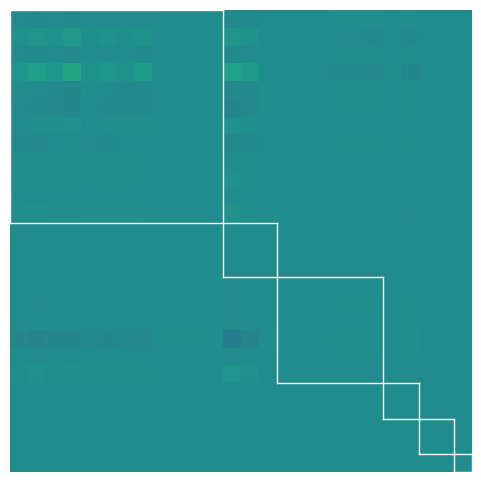
\includegraphics[width=0.22\linewidth]{kfac_pinns_exp/exp04_gramian_contributions/fig/gram_hess_input_output.png}
    &
      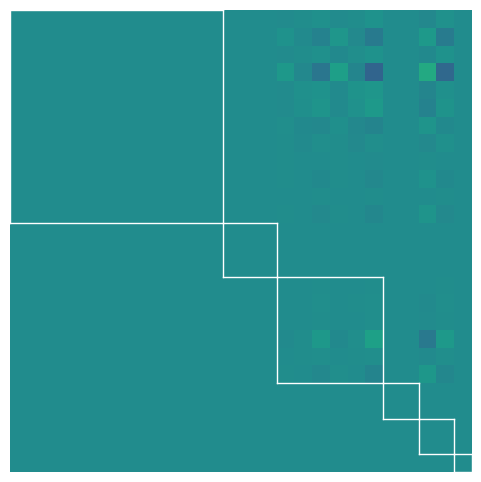
\includegraphics[width=0.22\linewidth]{kfac_pinns_exp/exp04_gramian_contributions/fig/gram_hess_input_grad_input.png}
    &
      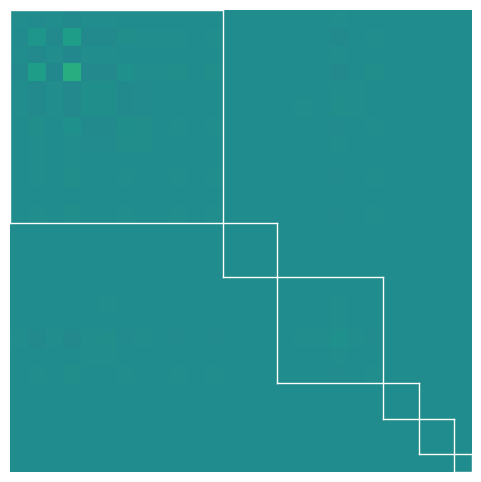
\includegraphics[width=0.22\linewidth]{kfac_pinns_exp/exp04_gramian_contributions/fig/gram_hess_input_hess_input.png}
  \end{tabular}
  \caption{Contributions $\mG_{\Omega,\textcolor{blue}{\bullet}, \textcolor{red}{\bullet}}$ to the Laplacian's Gramian $\mG_{\Omega}$ from different children in the computation graph on a synthetic toy problem.
    We use a $4 \to 3 \to 2 \to 1$ sigmoid-activated MLP and 10 randomly generated inputs. The contributions are highlighted as in \Cref{eq:fisher}.}\label{fig:gramian-contribution-children}
\end{figure}
%%% Local Variables:
%%% mode: latex
%%% TeX-master: "../main"
%%% End:


The Jacobians from \Cref{eq:fisher-jacobians} allow to express the Fisher in terms of Kronecker-structured expressions consisting of 9 terms in total.
For the off-diagonal terms, which stem from two different children, we combine the two terms that involve the same children into a symmetric term.
\Cref{fig:gramian-contribution-children} shows the resulting 6 terms.

\begin{figure}
  \centering
  Full Gramian\\
  \includegraphics[width=0.43\linewidth]{../kfac_pinns_exp/exp04_gramian_contributions/fig/gram_full.png}

  \begin{minipage}[t]{0.22\linewidth}
    \centering
    Block diagonal
    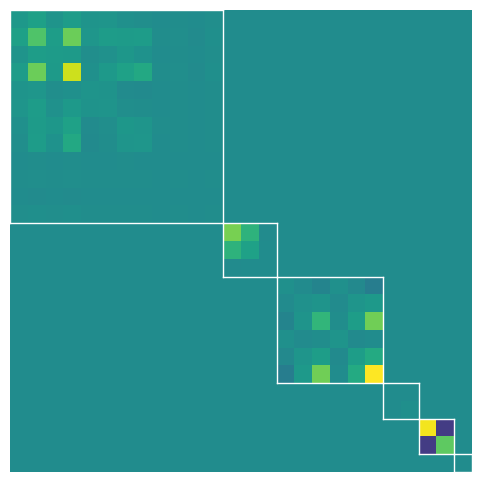
\includegraphics[width=\linewidth]{../kfac_pinns_exp/exp04_gramian_contributions/fig/gram_block_diag.png}
  \end{minipage}
  \hfill
  \begin{minipage}[t]{0.22\linewidth}
    \centering
    Summed children diagonal
    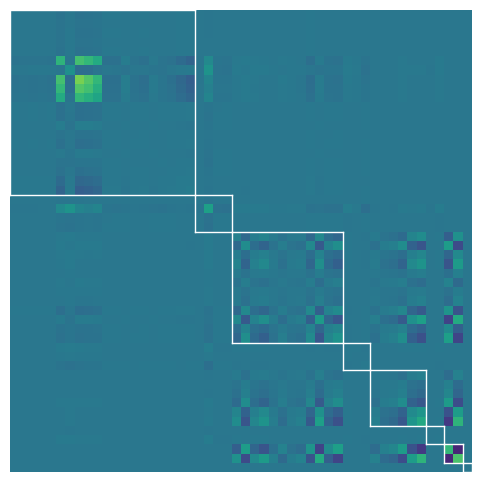
\includegraphics[width=\linewidth]{../kfac_pinns_exp/exp04_gramian_contributions/fig/gram_diag_children.png}
  \end{minipage}
  \hfill
  \begin{minipage}[t]{0.22\linewidth}
    \centering
    Summed children off-diagonal
    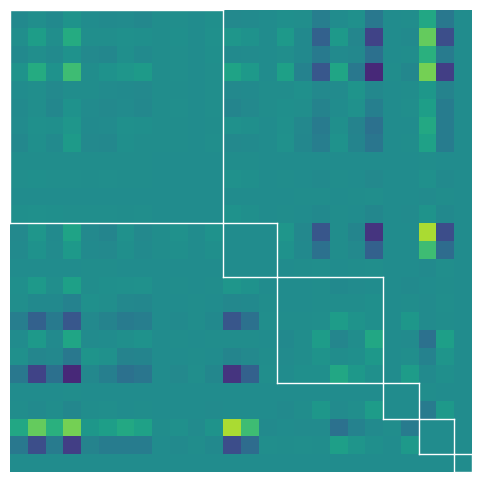
\includegraphics[width=\linewidth]{../kfac_pinns_exp/exp04_gramian_contributions/fig/gram_offdiag_children.png}
  \end{minipage}
  \caption{Contribution of terms with identical versus non-identical children to the Gramian's block diagonal.
    The strongest contribution to its block diagonal stems from the terms with identical children.}\label{fig:gramian-contribution-summed-children}
\end{figure}
%%% Local Variables:
%%% mode: latex
%%% TeX-master: "../main"
%%% End:


\Cref{fig:gramian-contribution-summed-children} shows an alternative comparison where we group the terms stemming from two identical and two different nodes (that is the diagonals and off-diagonals of \Cref{eq:fisher-jacobians}) into one matrix.
For the Gramian's block diagonal (leftmost panel), we can see that the contribution from identical nodes (center panel) is larger than that of different nodes (rightmost panel).
This is a first promising observation: Since we tackle the approximation of the Gramian's block diagonal, we can focus on the contributions from identical nodes.
These are also simpler to compute because they can be computed at one stage of backpropagation.

Some insights while creating \Cref{fig:hbp-dependencies} that might explain the structures of the Gramian displayed in \Cref{fig:gramian-contribution-children}:
\begin{itemize}
\item Assume the NN's first layer is a linear layer with weight matrix $\mW^{(1)}$.
  Then, we have that the Laplacian's derivative w.r.t.\, the input Hessian is
  \begin{equation*}
    \grad{\gradsquared{\vx}u}\Delta \vx = \flatten(\mI)\,.
  \end{equation*}
  This is because the relation between the two is taking the trace.
  Then, we can write down the (Hessian, Hessian) contribution to the Gramian
  exactly as
  \begin{align*}
    \mF^{(1)}_{\gradsquared{\vx}u, \gradsquared{\vx}u}
    &=
      \left\{
      2
      \left(
      \mI \otimes
      \left[
      \left( \gradsquared{\vz^{(1)}}u \right) \mW^{(0)}
      \right]
      \right)
      \flatten(\mI)
      \right\}
      \left\{
      2
      \left(
      \mI \otimes
      \left[
      \left( \gradsquared{\vz^{(1)}}u \right) \mW^{(0)}
      \right]
      \right)
      \flatten(\mI)
      \right\}^{\top}
    \\
    &=
      \left\{
      2
      \flatten
      \left(
      \mI \otimes
      \left[
      \left( \gradsquared{\vz^{(1)}}u \right) \mW^{(0)}
      \right]
      \right)
      \right\}
      \left\{
      2
      \flatten
      \left(
      \mI \otimes
      \left[
      \left( \gradsquared{\vz^{(1)}}u \right) \mW^{(0)}
      \right]
      \right)
      \right\}^{\top}
    \\
    &=
      \text{(F.D. Not sure if this can be further simplified.)}
  \end{align*}

\item If the last layer is a linear layer, it's weight does not contribute to the Hessian during the Hessian backward pass.
  This is because the incoming Hessian is $\gradsquared{u}u = \vzero$, and the Hessian backpropagation is $\gradsquared{\vz^{(L-1)}}u = {\mW^{(L)}}^T\vzero \mW^{(L)} = \vzero$.
  Only the activation layer before the last linear layer will start introducing curvature.
  Hence,
  \begin{align*}
    \grad{\mW^{(L)}} \Delta u
    &=
      2
      \left(
      \mI \otimes
      \left[
      \vzero \mW^{(L)}
      \right]
      \right)
      \grad{\gradsquared{\vz^{(L-1)}}} \Delta u
      =
      \vzero
  \end{align*}
  and the associated block in $ \mF^{(L)}_{\bullet, \gradsquared{\vz^{(L-1)}}u}, \mF^{(L)}_{\gradsquared{\vz^{(L-1)}}u, \bullet} $ is zero.
  We can see this effect clearly in the ($\bullet$, Hessian) and ($\bullet$, Hessian) panels of \Cref{fig:gramian-contribution-children} where either row or column blocks associated to the last layer's weight are zero.

  A similar argument implies that for a network consisting only of linear layers and ReLU activations, the Hessian backpropagation will be zero for all layers.
  Consequentially, the Laplacian will be $\vzero$.
  This makes sense because ReLU-activated networks are piece-wise linear~\cite{arora2018understanding}, hence their Laplacian vanishes almost everywhere.

\item So far we only discussed weights.
  Bias terms are even simpler because they only contribute in the forward pass, irrespective of which layer they reside in.
  They are not used in any operation of the backward and Hessian backward procedure.
  Hence, in all panels except for (forward, forward) of \Cref{fig:gramian-contribution-children} the row/column blocks associated with bias terms are zero.
\end{itemize}

\paragraph{Computing $\grad{\textcolor{blue}{\bullet}}\Delta u$}
The terms $\grad{\textcolor{blue}{\bullet}}\Delta u$ are automatically computed when computing the gradient of the loss via backdrop.

\paragraph{Zeroth order diagonal term}
Note that one of the nine terms is the term similar to the original KFAC paper, namely
when $\textcolor{blue}{\bullet} = \textcolor{red}{\bullet} = \vz^{(i)}$
(remember that $\jac_{\mW^{(i)}} \vz^{(i)} = \vz^{(i-1)} \otimes \mI$):
\begin{align}\label{eq:original-kfac}
  \begin{split}
    \mF^{(i)}_{\textcolor{blue}{\vz^{(i)}}, \textcolor{red}{\vz^{(i)}}}
    &=
      \left(
      \textcolor{blue}{\vz^{(i-1)} \otimes \mI}
      \right)
      \left[
      \left(
      \textcolor{blue}{\grad{\vz^{(i)}}\Delta u}
      \right)
      \left(
      \textcolor{red}{\grad{\vz^{(i)}}\Delta u}
      \right)^{\top}
      \right]
      \left(
      \textcolor{red}{{\vz^{(i-1)}}^{\top} \otimes \mI}
      \right)
    \\
    &=
      \textcolor{blue}{\vz^{(i-1)}}
      \textcolor{red}{{\vz^{(i-1)}}^{\top}}
      \otimes
      \left(
      \textcolor{blue}{\grad{\vz^{(i)}}\Delta u}
      \right)
      \left(
      \textcolor{red}{\grad{\vz^{(i)}}\Delta u}
      \right)^{\top}
    \\
    &\coloneqq \mA_{\text{KFAC}}^{(i)} \otimes \mB_{\text{KFAC}}^{(i)}\,.
  \end{split}
\end{align}
Note however, that in comparison to traditional KFAC, there are Laplacian terms.
\Cref{eq:original-kfac} illustrates that the Kronecker structure emerges from
the Jacobians. So we need to investigate these objects closer for the remaining
terms of \Cref{eq:fisher}.


\paragraph{First order diagonal term}

\paragraph{Second order diagonal term}


%%% Local Variables:
%%% mode: latex
%%% TeX-master: "../main"
%%% End:
